% arara: lualatex
\documentclass{standalone}
\usepackage{mathtools}
\usepackage{unicode-math}
\unimathsetup{math-style=TeX}
\setmainfont{TeX Gyre Pagella}
\setmathfont{TeX Gyre Pagella Math}
\usepackage[version=3]{mhchem}
\usepackage{chemfig}
\setatomsep{2.25em}
\usetikzlibrary{positioning, calc, arrows.meta}
\tikzset{
    flux/.style={
        flux/.cd,
        #1,
        print,
    },
    flux/.cd,
    position/.store in=\position,
    position=0.6,
    fluxabove/.store in=\fluxabove,
    fluxbelow/.store in=\fluxbelow,
    print/.style={
        /tikz/.cd,
        insert path={%
            node [pos=\position, above] {\SI{\fluxabove}{\percent}} node[pos=\position, below] {\textbf{\SI{\fluxbelow}{\percent}}}%
        },
    },
}
\usepackage{siunitx}
\sisetup{detect-all=true}

\begin{document}
    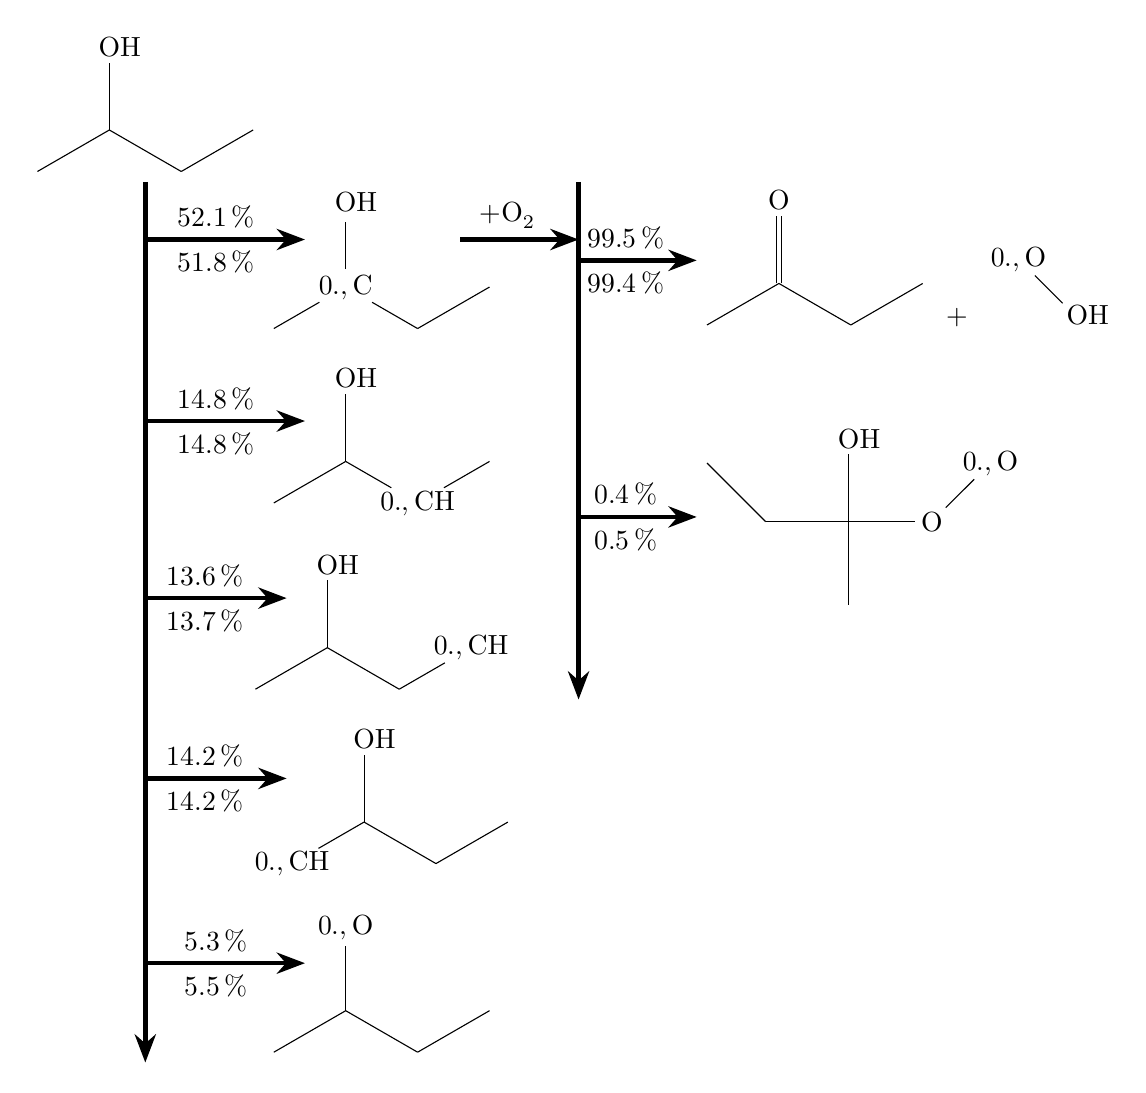
\begin{tikzpicture}[x=1cm, y=1cm]
        \begin{scope}[every node/.style={node distance=0.25}]
            \node (sbuoh) {\chemfig{-[:30](-[2]OH)-[:330]-[:30]}};
            \node[below right=0 and 0 of sbuoh] (asbuoh) {\chemfig{-[:30]\lewis{0.,C}(-[2]OH)-[:330]-[:30]}};
            \node[below=of asbuoh] (b1sbuoh) {\chemfig{-[:30](-[2]OH)-[:330]\lewis{0.,CH}-[:30]}};
            \node[below=of b1sbuoh] (gsbuoh) {\chemfig{-[:30](-[2]OH)-[:330]-[:30]\lewis{0.,CH}}};
            \node[below=of gsbuoh] (b2sbuoh) {\chemfig{\lewis{0.,CH}-[:30](-[2]OH)-[:330]-[:30]}};
            \node[below=of b2sbuoh] (osbuoh) {\chemfig{-[:30](-[2]\lewis{0.,O})-[:330]-[:30]}};
            \node[right=2.5 of asbuoh] (sbuohalde) {\chemfig{-[:30](=[2]O)-[:330]-[:30]} \, $+$ \, \chemfig[baseline=(a)]{\lewis{0.,O}-[7]OH@{a}}};
            \node[below left=1 and 0 of sbuohalde, anchor=north west] (asbuohoo) {\chemfig{-[7]-(-[2]OH)(-[6])-O-[1]\lewis{0.,O}}};
        \end{scope}

        \begin{scope}[every path/.style={draw, ultra thick, >={Stealth}}]
            \path[->] let \p1 = (sbuoh.south), \p2 = (osbuoh.south) in (\x1,\y1) -- (\x1,\y2) coordinate (lineend);
            \path[->, shorten >=-15] ($(sbuoh.south)!(asbuoh.170)!(lineend)$) -- (asbuoh.170) [flux={fluxabove=52.1, fluxbelow=51.8}];
            \path[->, shorten >=-15] ($(sbuoh.south)!(b1sbuoh.170)!(lineend)$) -- (b1sbuoh.170) [flux={fluxabove=14.8, fluxbelow=14.8}];
            \path[->, shorten >=-15] ($(sbuoh.south)!(gsbuoh.170)!(lineend)$) -- (gsbuoh.170) [flux={fluxabove=13.6, fluxbelow=13.7}];
            \path[->, shorten >=-15] ($(sbuoh.south)!(b2sbuoh.170)!(lineend)$) -- (b2sbuoh.170) [flux={fluxabove=14.2, fluxbelow=14.2}];
            \path[->, shorten >=-15] ($(sbuoh.south)!(osbuoh.170)!(lineend)$) -- (osbuoh.170) [flux={fluxabove=5.3, fluxbelow=5.5}];
            \coordinate (midline) at ($(asbuoh.east)!0.4!(sbuohalde.west)$);
            \path[->] let \p1 = (sbuoh.south), \p2 = (midline), \p3 = (gsbuoh.south) in (\x2,\y1) -- (\x2,\y3) coordinate (midlineend);
            \path[->] ($(midline)!(sbuohalde.west)!(midlineend)$) -- (sbuohalde.west) [flux={fluxabove=99.5, fluxbelow=99.4, position=0.4}];
            \path[->] ($(midline)!(asbuohoo.west)!(midlineend)$) -- (asbuohoo.west) [flux={fluxabove=0.4, fluxbelow=0.5, position=0.4}];
            \path[->] ($(asbuoh.10)-(0.5,0)$) -- ($(midline)!(asbuoh.10)!(midlineend)$) node[above, pos=0.4] {$+$\ce{O2}};
        \end{scope}
    \end{tikzpicture}
\end{document}
